%!TEX program = <xelatex>
% !Mode:: "TeX:UTF-8"

\documentclass[13pt]{beamer}
\usepackage{appendixnumberbeamer}
\usepackage{epigraph}
%\usepackage{ulem}
\usepackage{booktabs}
%\usepackage{cite}
\usepackage{listings}
\usepackage{color}
\usepackage{xcolor}
\usepackage{hyperref}
\usepackage[round]{natbib}
\usepackage{movie15}
\usepackage{animate}
\usepackage{mathtools}
\usepackage{threeparttable}
\setbeamertemplate{theorems}[numbered]
\setbeamertemplate{lemma}[numbered]
\setbeamertemplate{caption}[numbered]
\mode<presentation>
{
%\setbeamertemplate{background canvas}[vertical shading][bottom=red!10,top=blue!80]
\useoutertheme{infolines}
%\usetheme{Darmstadt}
%\setbeamertemplate{navigation symbols}{}
%\usecolortheme[RGB={165,42,42}]{structure}
\usetheme{default}
%\usetheme{IAS_sidebar} 	% only a simple left side bar, frame-title box varies in size when using subtitles for frames.
%\usetheme{IAS_sidebar2_10pt} 	% only a simple side bar, the frame-title box has a fixed size to exactly fit a title and subtitle. For usage with 10pt font, i.e.: \documentclass[10pt]{beamer}
%\usetheme{IAS_sidebar2_11pt} 	% As above only changed to fit 11pt fonts.
%\usetheme{IAS_sidebar2_12pt} 	% As above only changed to fit 12pt fonts.
%\usetheme{IAS_sidebarNav} 	% An IAS side bar with navigation
%\usetheme{IAS_topNav}		% Only top navigation with IAS colors
%\usetheme{IAS_topNav_bottomAuthorTitle}	%Top navigation and author/title in the bottom with IAS colors
%\usetheme{IAS_topNav_leftIASbar_10pt}	% both top navigation and the IAS sidebar, the frame-title box has a fixed size to exactly fit a title and subtitle. For usage with 10pt font, i.e.: \documentclass[10pt,english
%\usetheme{IAS_topNav_leftIASbar_11pt}	% As above only changed to fit 11pt fonts.
%\usetheme{IAS_topNav_leftIASbar_12pt}	% As above only changed to fit 12pt fonts.
  \setbeamercovered{transparent}
%   % or whatever (possibly just delete it)
% to remove the navigation symbols:
%\setbeamertemplate{navigation symbols}{}
}
\usepackage[english]{babel}
% or whatever

\usepackage[latin1]{inputenc}
% or whatever

\usepackage{times}
\usepackage[T1]{fontenc}
% Or whatever. Note that the encoding and the font should match. If T1
% does not look nice, try deleting the line with the fontenc.


\definecolor{Black}{RGB}{0,0,0}
\definecolor{Red}{RGB}{255,0,0}
\definecolor{Green}{RGB}{0,255,0}
\definecolor{Orange}{RGB}{255,165,0}
\definecolor{Cyan}{RGB}{0,255,255}
\definecolor{Yellow}{RGB}{255,255,0}
\definecolor{White}{RGB}{255,255,255}
\lstset
{
    breaklines=true,
    tabsize=3,
    showstringspaces=false
}


\lstdefinestyle{Common}
{
    extendedchars=\true,
    language={[Visual]Basic},
    frame=single,
    %===========================================================
    framesep=3pt,%expand outward.
    framerule=0.4pt,%expand outward.
    xleftmargin=3.4pt,%make the frame fits in the text area. 
    xrightmargin=3.4pt,%make the frame fits in the text area.
    %=========================================================== 
    rulecolor=\color{Red}
}

\lstdefinestyle{A}
{
    style=Common,
    backgroundcolor=\color{Yellow!10},
    basicstyle=\color{Black}\ttfamily,
    keywordstyle=\color{Orange},
    identifierstyle=\color{Cyan},
    stringstyle=\color{Red},
    commentstyle=\color{Green}
}

\lstdefinestyle{B}
{
    style=Common,
    backgroundcolor=\color{Black},
    basicstyle=\color{White}\ttfamily,
    keywordstyle=\color{Orange},
    identifierstyle=\color{Cyan},
    stringstyle=\color{Red},
    commentstyle=\color{Green}
}



\title[To JY.Z. \& JY.Y.] % (optional, use only with long paper titles)
{Excel VBA Foundation I}



\author[SHENG Hao] % (optional, use only with lots of authors)
{SHENG Hao\inst{1}}
% - Give the names in the same order as the appear in the paper.
% - Use the \inst{?} command only if the authors have different
%   affiliation.

\institute[GSM, PKU] % (optional, but mostly needed)
{
  \inst{1}%
  Guanghua School of Management,\\
  Peking University
}
% - Use the \inst command only if there are several affiliations.
% - Keep it simple, no one is interested in your street address.

\date[\today] % (optional, should be abbreviation of conference name)
{ At HEC Paris, Mar. 2015}
% - Either use conference name or its abbreviation.
% - Not really informative to the audience, more for people (including
%   yourself) who are reading the slides online

\subject{Personal Workshop in HEC}
% This is only inserted into the PDF information catalog. Can be left
% out.


% If you have a file called "university-logo-filename.xxx", where xxx
% is a graphic format that can be processed by latex or pdflatex,
% resp., then you can add a logo as follows:

\pgfdeclareimage[height=0.7cm]{university-logo}{ppelogo}
\logo{\pgfuseimage{university-logo}\hspace{15pt}\vspace{215pt}}
%\pgfdeclareimage[height=0.2cm]{institution-logo}{pkuword}
%\logo{\pgfuseimage{institution-logo}}



% Delete this, if you do not want the table of contents to pop up at
% the beginning of each subsection:
\AtBeginSubsection[]
{
  \begin{frame}<beamer>
    \frametitle{Outline}
    \tableofcontents[currentsection,currentsubsection]
  \end{frame}
}


% If you wish to uncover everything in a step-wise fashion, uncomment
% the following command:

%\beamerdefaultoverlayspecification{<+->}



\begin{document}

\DeclarePairedDelimiter{\ceil}{\lceil}{\rceil}


\begin{frame}
  \titlepage
\end{frame}

\addtocounter{framenumber}{-1}
\begin{frame}
  \frametitle{Outline}
  \tableofcontents
  % You might wish to add the option [pausesections]
\end{frame}

% Structuring a talk is a difficult task and the following structure
% may not be suitable. Here are some rules that apply for this
% solution:

% - Exactly two or three sections (other than the summary).
% - At *most* three subsections per section.
% - Talk about 30s to 2min per frame. So there should be between about
%   15 and 30 frames, all told.

% - A conference audience is likely to know very little of what you
%   are going to talk about. So *simplify*!
% - In a 20min talk, getting the main ideas across is hard
%   enough. Leave out details, even if it means being less precise than
%   you think necessary.
% - If you omit details that are vital to the proof/implementation,
%   just say so once. Everybody will be happy with that.
\section{Preview}

\begin{frame}[t]
  \frametitle{Preview}
  \begin{flushright}
    {\sc To the time to life, rather than to life in time.\\}%
  	{\sc---Blaise Pascal}
  \end{flushright}

  \vspace{30pt}

  \begin{itemize}
  \item Take-aways:
  \begin{itemize}
  		\item Basic concepts in VBA \pause
      \item Tools in coding \pause
      \item Specific coding cases \pause
      \begin{itemize}
        \item Data Formating \pause
        \item Modeling \pause
        \item Data Visualization 
      \end{itemize}
 \end{itemize}
  \end{itemize}
  \vspace{80pt}
\end{frame}

\section{About This Seminar}
\begin{frame}[t]\frametitle{About This Seminar}
\begin{itemize}
  \item Main topics 
  \begin{itemize}
    \item Writing Excel Macros with VBA, 2e \\
    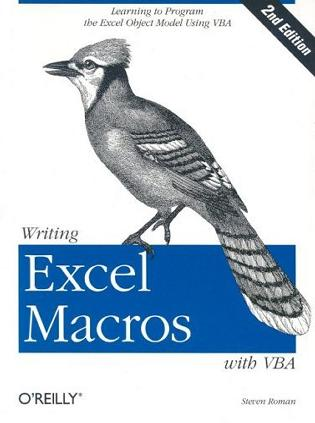
\includegraphics[width=0.25\textwidth]{Reilly.jpg}
    
  \end{itemize}
  \item Coding (2-5 cases each time)
    \begin{itemize}
     \item Excel VBA in 150 programs
    \end{itemize}
  \item Real problems

\end{itemize}
  
\end{frame}

\section{Programing Language and VBA}

\subsection{Programing Language}
\begin{frame}[t]\frametitle{Programing Language}
    \begin{itemize}
    	\item Languages designed to manipulate the computer at a low level, that is, to manipulate the operating system (Windows or DOS) or even the hardware itself, are called low-level languages. \pause
    	\begin{itemize}
    		\item Assembly language
    	\end{itemize}
      \pause

    	\item Languages designed to create standalone applications, such as Microsoft Excel, are high-level languages. \pause
    	\begin{itemize}
    		\item BASIC and Pascal \pause
    		\item C, C++, VB, Python \pause
    		\item MATLAB, Mathematica, R, SAS, Stata \pause
    	\end{itemize} 
      \pause

    	\item Languages that are designed to manipulate an application program, such as Microsoft Excel, are application-level languages. \pause
    	\begin{itemize}
    	 	\item Excel VBA, Word VBA, and PowerPoint VBA
    	 \end{itemize} 
    \end{itemize}

\end{frame}

\subsection{Programing Style}
\begin{frame}[t]\frametitle{Programing Style}
	\begin{itemize}
		\item Comments
		\item Readability
		\item Modularity
		\begin{itemize}
			\item Next slide
		\end{itemize}
	\end{itemize}

\end{frame}


\begin{frame}[t]\frametitle{Programing Style}\framesubtitle{Modularity}
\begin{itemize}
	\item In one program
\end{itemize}
 \lstinputlisting[style = B, basicstyle=\tiny]{VBA1.txt}
\end{frame}

\begin{frame}[t]\frametitle{Programing Style}\framesubtitle{Modularity (cont.)}
\begin{itemize}
	\item Main program
\end{itemize}
 \lstinputlisting[style = B, basicstyle=\tiny]{VBA2.txt}
\begin{itemize}
	\item Modular
\end{itemize}
 \lstinputlisting[style = B, basicstyle=\tiny]{VBA3.txt}

\end{frame}

\section{By Example (Application Object)}
\subsection{StatusBar}
\begin{frame}[t]\frametitle{StatusBar}
     \lstinputlisting[style = B, basicstyle=\tiny]{VBA4.txt}
\end{frame}
\subsection{FullScreen and Exit}
\begin{frame}[t]\frametitle{FullScreen and Exit}
     \lstinputlisting[style = B, basicstyle=\tiny]{VBA5.txt}
\end{frame}
\subsection{Onkey}
\begin{frame}[t]\frametitle{Onkey}
     \lstinputlisting[style = B, basicstyle=\tiny]{VBA6.txt}
\end{frame}

\section*{Reference}
\begin{frame}[allowframebreaks]
	\frametitle{Reference}
	\bibliographystyle{jpe}
	\bibliography{Excelbib}
	\nocite{*}
\end{frame}

\end{document}



